\tikzset{>=latex} % for LaTeX arrow head
\contourlength{1.1pt}

\colorlet{xcol}{blue!98!black}
\colorlet{xcoldark}{blue!50!black}
\colorlet{vcol}{green!70!black}
\colorlet{myred}{red!80!black}
\colorlet{mypurple}{blue!60!red!80}
\colorlet{acol}{red!50!blue!80!black!80}
\tikzstyle{rvec}=[->,xcol,very thick,line cap=round]
\tikzstyle{force}=[->,myred,very thick,line cap=round]
\tikzstyle{mass}=[line width=0.6,red!30!black,fill=red!40!black!10,rounded corners=1,
                  top color=red!40!black!20,bottom color=red!40!black!10,shading angle=20]

\tikzset{
  pics/Tin/.style={
    code={
      \def\R{0.12}
      \draw[pic actions,line width=0.6,#1,fill=white] % ,thick
        (0,0) circle (\R) (-135:.75*\R) -- (45:.75*\R) (-45:.75*\R) -- (135:.75*\R);
  }},
  pics/Tout/.style={
    code={
      \def\R{0.12}
      \draw[pic actions,line width=0.6,#1,fill=white] (0,0) circle (\R);
      \fill[pic actions,#1] (0,0) circle (0.3*\R);
  }},
  pics/Tin/.default=mypurple,
  pics/Tout/.default=mypurple,
}

\newcommand\rightAngle[4]{
  \pgfmathanglebetweenpoints{\pgfpointanchor{#2}{center}}{\pgfpointanchor{#3}{center}}
  \coordinate (tmpRA) at ($(#2)+(\pgfmathresult+45:#4)$);
  \draw[white,line width=0.7] ($(#2)!(tmpRA)!(#1)$) -- (tmpRA) -- ($(#2)!(tmpRA)!(#3)$);
  \draw[xcoldark] ($(#2)!(tmpRA)!(#1)$) -- (tmpRA) -- ($(#2)!(tmpRA)!(#3)$);
}

\def\r{0.16}  % axis radius
\def\Ri{1.18} % wheel rims inside
\def\Rr{1.30} % wheel rims outside
\def\Rt{1.45} % wheel tyre
\def\wheel{
  \def\Ns{11}   % number of spokes
  \def\Nn{34}   % number of tyre stud
  \coordinate (O) at (0,0);
  \foreach \i [evaluate={\ang=\i*360/(\Ns+1);}] in {0,...,\Ns}{
    \draw[line width=0.5,black!70,line cap=round] (\ang-90:\r) --++ (\ang:\Rr);
  }
  \draw[very thin,fill=black!30] (O) circle (1.2*\r);
  \draw[very thin,black!70] (O) circle (0.6*\r) circle (0.3*\r);
  \foreach \i [evaluate={\ang=\i*360/(\Ns+1);}] in {0,...,\Ns}{
    \fill (\ang+90:\r) circle (0.015);
    \draw[line width=0.5,black!70,line cap=round] (\ang+90:\r) --++ (\ang:\Rr);
  }
  \draw[fill=black!30,even odd rule] (O) circle (\Ri) circle (\Rr);
  
  \draw[fill=black!84,even odd rule] (O) circle (\Rr) (\Rt,0)
    \foreach \i [evaluate={\anga=\i*360/(\Nn+1);\angb=(\i+0.5)*360/(\Nn+1);
                           \angc=(\i+1)*360/(\Nn+1);}] in {0,...,\Nn}{
      -- (\anga:1.008*\Rt) arc(\anga:\angb:1.008*\Rt)
      -- (\angb:1.000*\Rt) arc(\angb:\angc:1.000*\Rt)
    } -- cycle;
  \draw[very thin] (O) circle (0.97*\Rt) circle (0.945*\Rt);
}

% TORQUE perpendicular
\def\R{1.6} % wheel rims inside




% TORQUE parallel


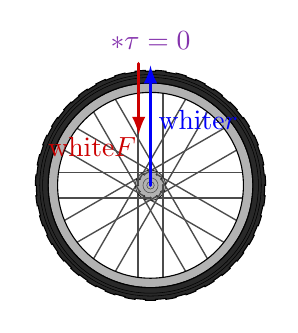
\begin{tikzpicture}
  \def\ang{90} % angle
  \def\F{0.9}  % force size
  \coordinate (O) at (0,0);
  \coordinate (R) at (\ang:\R);
  \clip (-1.2*\Rr,-1.17*\Rr) rectangle (1.17*\Rr,1.54*\Rr);
  \wheel
  \node[mypurple,above=0] at (R) {$\vb*\tau = 0$};
  \draw[force] (R)++(\ang+110:0.16) --++ (\ang-180:\F) node[below left=-3] {\contour{white}{$\vb{F}$}};
  \draw[rvec] (O) -- (\ang:0.95*\R) node[midway,above=2,right=-1] {\contour{white}{$\vb{r}$}};
\end{tikzpicture}
